\subsection{Calorimeter}
\label{sec:Det:Cal}

\begin{figure}
  \centering
  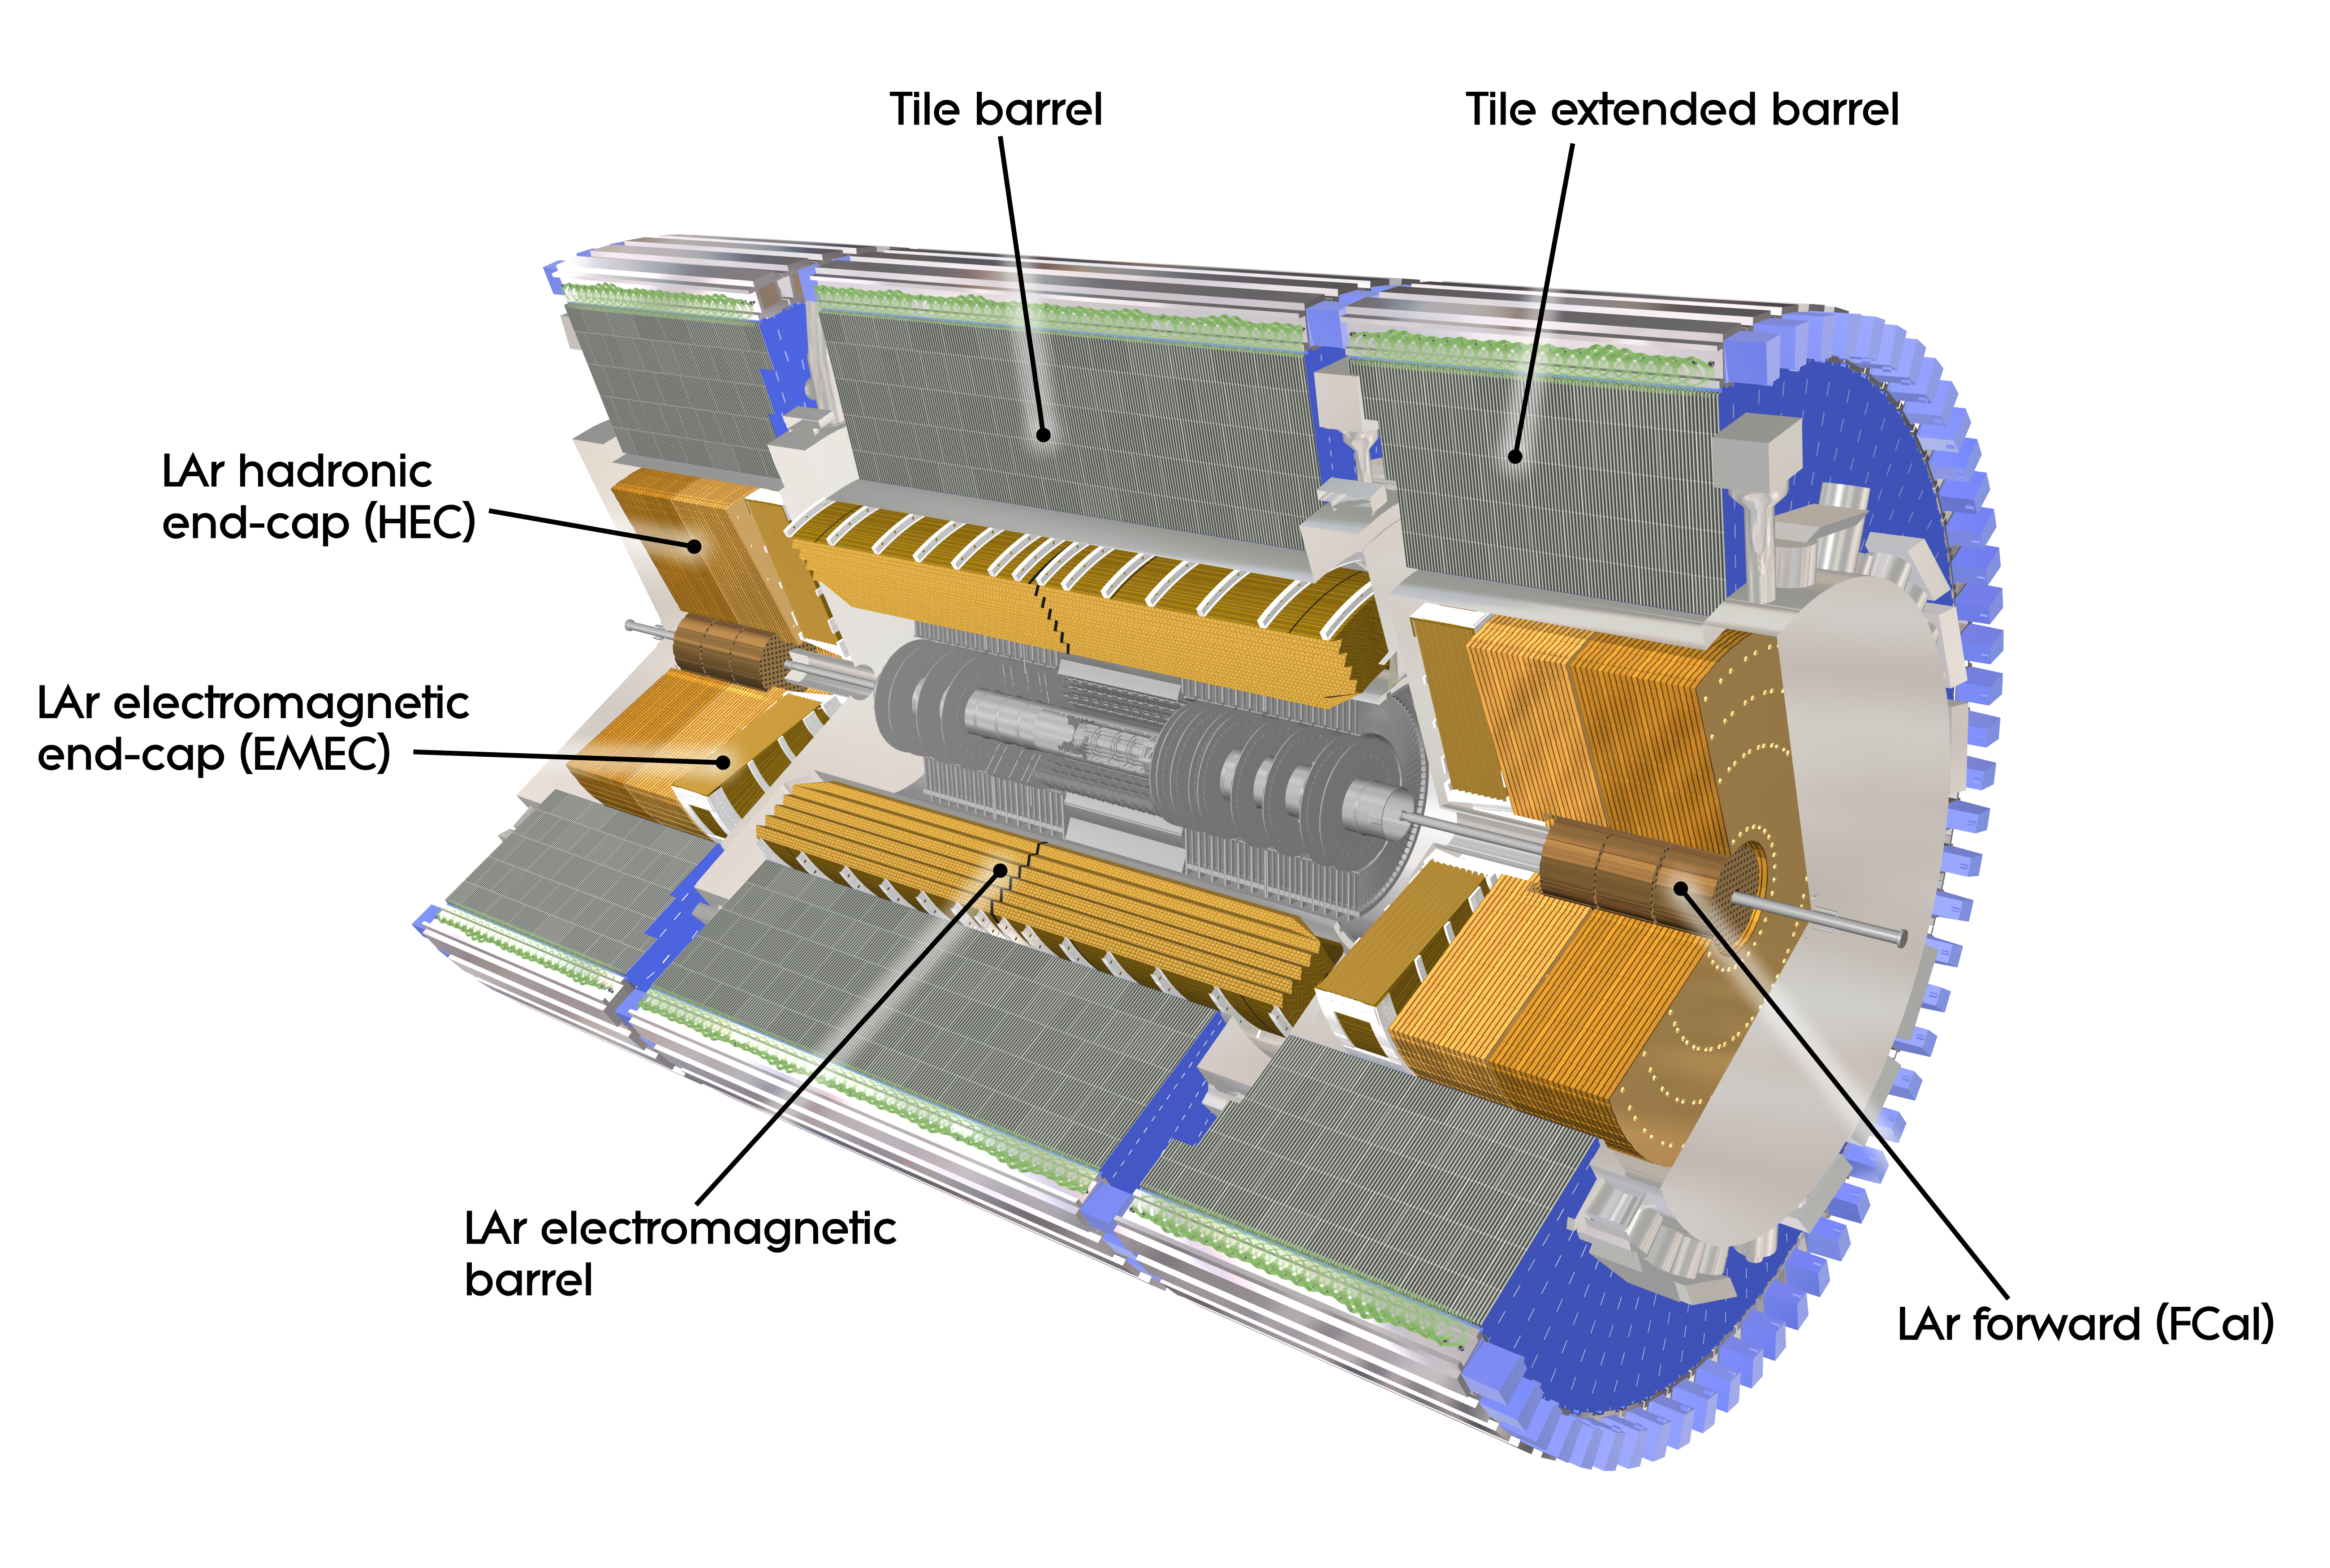
\includegraphics[width=0.9\textwidth]{figures/Detector/AtlasCalorimeter.jpg}
  \caption{ATLAS calorimeter system.}
\label{Det:ATLASCalo}
\end{figure}

This section will discuss the EM calorimeter, the hadronic calorimeter and the forward calorimeter. 
The ATLAS calorimeter system comprises several sampling detectors which have a complete $\phi$ coverage.
With the exception of the barrel hadronic calorimeter (Tile barrel and extended barrel) all use LAr as the active material due to the radiation hardness and regularity of response.

\subsubsection{EM Calorimeter}

The EM calorimeter consists of a barrel detector and two end cap detectors, which together gives a coverage of $|\eta|<3.2$.
Figure \ref{Det:ATLASCalo} shows the EM barrel and the EM end cap, which have the pseudorapidity range $|\eta|<1.475$ and $1.375<|\eta|<3.2$ respectively.
In the precision region,  which is the region that overlaps the inner detector ($|\eta|<2.5$), there are three active layers and the detector is finely granulated to give a precise position measurement of the EM shower (used for photons).
Outside of the precision region there are two active layers and the granularity is coarser. 
The EM calorimeter has greater than 22 radiation lengths to attempt to fully contain any EM showers.


\subsubsection{Hadronic Calorimeter}

The hadronic calorimeter consists of three tile calorimeters (one barrel and two extended barrel) in the region $|\eta|<1.7$ and two hadronic end caps (HEC) to extend the coverage to $|\eta|<3.2$ as shown in Figure \ref{Det:ATLASCalo}.  

The HEC has two wheels per end cap, each with 32 wedged-shaped modules. 
The HEC has a granulation of $\Delta\eta \rm{x} \Delta\Phi = 0.1\rm{x}0.1$ in the region $|\eta|<2.5$ and $\Delta\eta \rm{x} \Delta\Phi = 0.2\rm{x}0.2$ in the region $2.5<|\eta|<3.2$. 
Each wheel has two different depth segments, resulting in four layers per end cap.


The tile calorimeter has three components, one barrel and two extended barrels. 
The tile barrel and tile extended barrel cover the range $|\eta|<1$ and $0.8<|\eta|<1.7$ respectively. 
These detectors comprise 64 modules which have a size of $\Delta\phi$~0.1, resulting in a granularity of $\Delta\eta \rm{x} \Delta\Phi = 0.1\rm{x}0.1$.

\subsubsection{Forward Calorimeter}

The forward calorimeter (fcal), shown in Figure \ref{fig:ATLASCalo}, is responsible for measuring the EM and hadronic showers in the region $3.2<|\eta|<4.9$.
The fcal has three detecting layers. 
The first layer is made of copper that is optimised for EM measurements.
This is followed by two tungsten layers used to measure hadronic energy deposits. 
All layers have LAr as the active material. 
The choice of materials and design was largely determined by the need to be radiation hard to withstand the  high particle flux.


\subsubsection{Calorimeter Objects}

To help construct photons, electons, taus or jets, an algorithm to cluster calorimeter cells is used. 
The aim of clustering is to reconstruct the 3D shower from the calorimeter cells. 
Clusters are formed by first finding a cluster seed, which is a cell with $|E|>4\sigma_{noise}$, where $\sigma_{noise}$ is ... 
The cluster is then extended by including all cells next to it with $|E|>2\sigma_{noise}$. 
An additional layer of cells with $|E|>0\sigma_{noise}$ are included. 
The advantage of using this clustering rather than towers (groups of cells at fixed $\Delta\eta\Delta\phi$) is to improve noise suppression.

%https://twiki.cern.ch/twiki/pub/Atlas/TapmJet/jetslice_v3_6April08.pdf


